%!TEX root = main.tex

\subsection{Dataset}

In this project, we  use NIST Special Database 4 \cite{nist-db-4} and NIST Special Database 14 \cite{nist-db-14} for our experiments. Some samples can be seen in Fig.\ref{fig.fingerprint_classes}.
%
The NIST SD4 contains $2000$ 8-bit gray scale fingerprint image pairs, totally 4000 images.
%
The size of each image is $512\times512$ and each image is classified using one of the five following classes: Arch, Left and Right Loops, Tented Arch, Whorl.
%
Each of the five classes has 400 pairs(800 images). Each of the fingerprint pairs are two completely different rollings of the same fingerprint.

%
The NIST SD14 contains $27000$ 8-bit gray scale fingerprint image pairs. There are 2700 subjects in this dataset and each subject has 10 fingerprint samples pairs. The size of each image is  $768\times832$. To fit in our network, we centrally crop $768\times768$ from the samples and resize them into $512\times512$. The distribution of fingerprint classes is as shown in Table.\ref{tab.sd14_dist}.


\begin{table}[!ht]
	\centering
	\caption{Class Distribution of NIST SD14.}
\label{tab.sd14_dist}
	\begin{tabular}{|c|c|c|c|c|}
		\hline
		\textbf{Arch} & \textbf{Left Loop} & \textbf{Right Loop} & \textbf{\begin{tabular}[c]{@{}c@{}}Tented \\ Arch\end{tabular}} & \textbf{Whorl} \\ \hline
		3.6\% & 31.9\% & 30.5\% & 3.2\% & 30.8\% \\ \hline
	\end{tabular}
\end{table}

\subsection{Experimental Setup}
We use a i7-5930K desktop with 32GB memory and a Nvidia GTX TITAN X GPU for experiments.
%
Typically, we use tensorflow 1.0.1 as the deep learning library and Adaptive Moment Estimation(Adam\cite{kingma2014adam}) as the optimization algorithm. The leaning rate is 0.0001. We also use $\ell_2$ regularization with 0.0001 weight decay rate. The batch size is 32. We run $20k$ steps and report the results.

We evaluate our approach on NIST SD4 and NIST SD14 respectively.
%
For NIST SD14 experiments, we use the samples of 80\% subjects for training, totally 2160 subjects with $43200$ images. Among these $432000$ images, 36 of them have labels that do not belong to the 5 classes. These 36 images are discarded. 
The remained data of 20\% subjects are used for testing, totally $10800$ images. 9 of these images are discarded due to the same reason above.
%

For NIST SD4 experiments, we first use NIST SD14 data to pre-train the model. Then we use all the first samples (2000) in each image pair as training samples and all the second samples (2000) for testing.
%


In addition to 5-class fingerprint classification, we also evaluate our approach on 4-class fingerprint classification because 4 class classification are also used in other studies. 
%
To achieve 4-class classification, we merge tented arch class into arch class when training SVM.

\begin{figure*}[!ht]
	\begin{subfigure}[b]{0.25\textwidth}
		\centering
		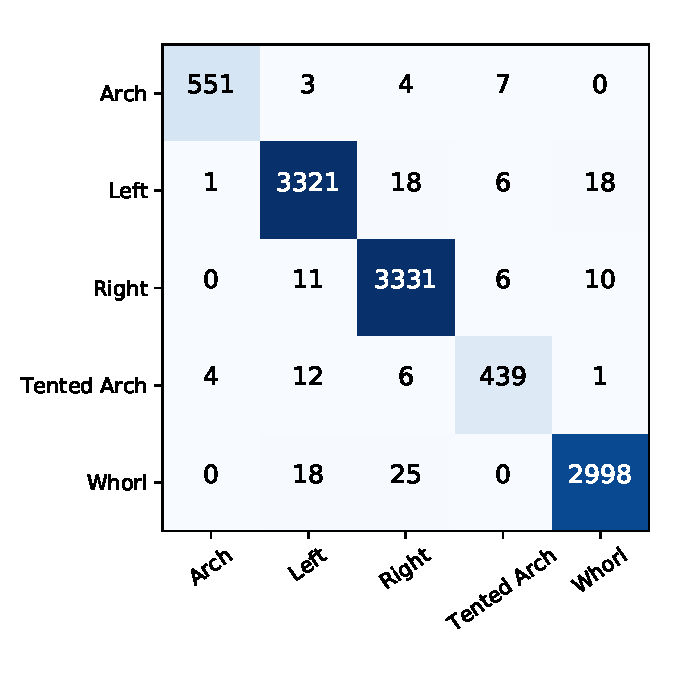
\includegraphics[width=\linewidth]{fig/figs/confusion_matrix_svm_sd14.pdf}
		\caption{SVM NIST SD14 }
		\label{fig.cnf_matrix_5class.svm_sd14}
	\end{subfigure}%
	\begin{subfigure}[b]{0.25\textwidth}
		\centering
		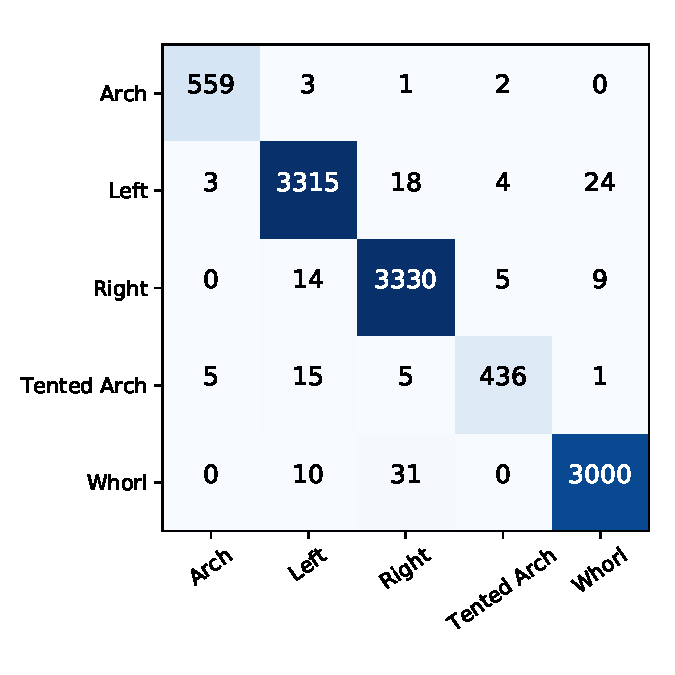
\includegraphics[width=\linewidth]{fig/figs/confusion_matrix_net_sd14.pdf}
		\caption{ConvNet NIST SD14 }
		\label{fig.cnf_matrix_5class.net_sd14}
	\end{subfigure}%
	\begin{subfigure}[b]{0.25\textwidth}
		\centering
		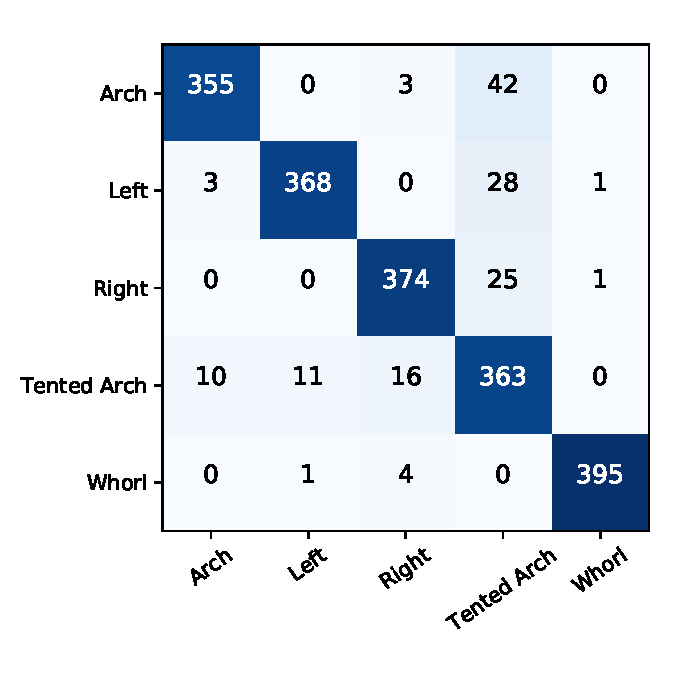
\includegraphics[width=\linewidth]{fig/figs/confusion_matrix_svm_sd4.pdf}
		\caption{SVM NIST SD4 }
		\label{fig.cnf_matrix_5class.svm_sd4}
	\end{subfigure}%
	\begin{subfigure}[b]{0.25\textwidth}
		\centering
		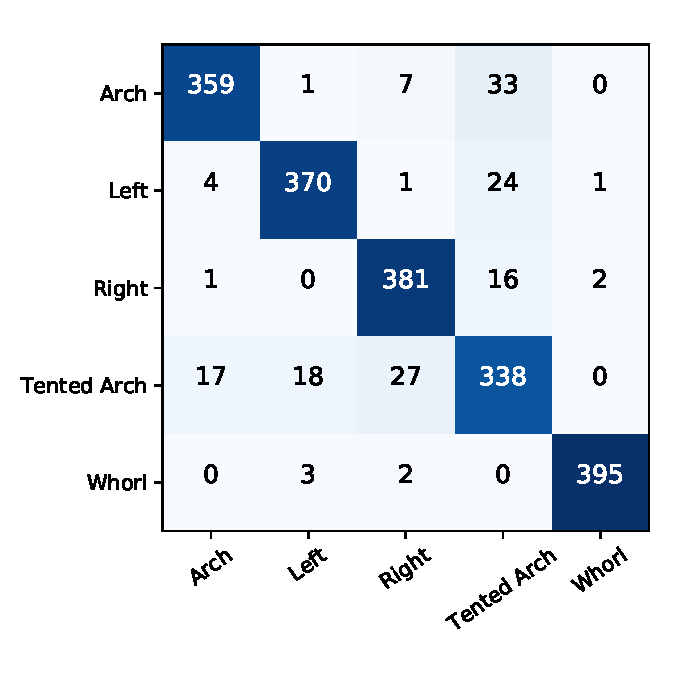
\includegraphics[width=\linewidth]{fig/figs/confusion_matrix_net_sd4.pdf}
		\caption{ConvNet NIST SD4 }
		\label{fig.cnf_matrix_5class.net_sd4}
	\end{subfigure}
	\caption{Confusion Matrices for 5-class classification}\label{fig.cnf_matrix_5class}
\end{figure*}

\begin{figure}[!ht]
	\begin{subfigure}[b]{0.25\textwidth}
		\centering
		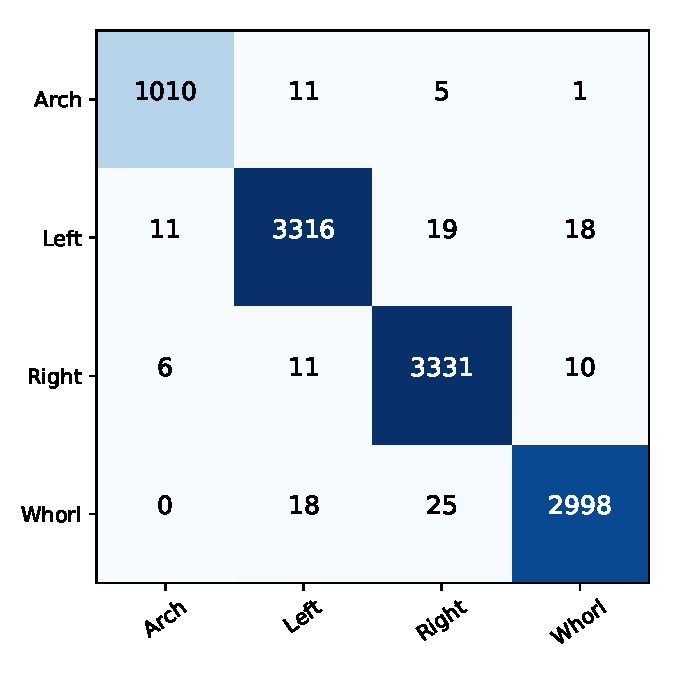
\includegraphics[width=\linewidth]{fig/figs/confusion_matrix_svm_sd14_4class.pdf}
		\caption{SVM NIST SD14 }
		\label{fig.cnf_matrix_4class.svm_sd14}
	\end{subfigure}%
	\begin{subfigure}[b]{0.25\textwidth}
		\centering
		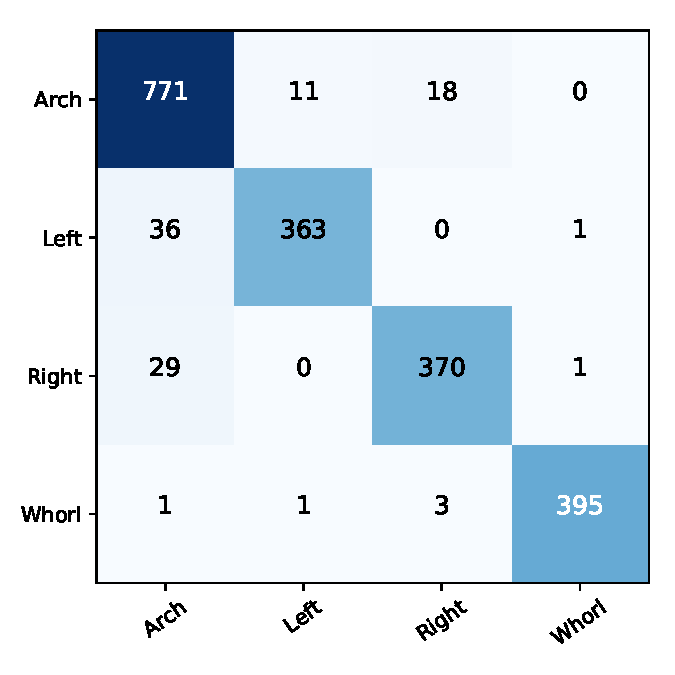
\includegraphics[width=\linewidth]{fig/figs/confusion_matrix_svm_sd4_4class.pdf}
		\caption{SVM NIST SD4}
		\label{fig.cnf_matrix_4class.svm_sd4}
	\end{subfigure}%

	\caption{Confusion Matrices for 4-class classification}\label{fig.cnf_matrix_4class}
\end{figure}

\subsection{NIST SD14 result}
The result for NIST SD14 is shown in Table\ref{tab.SD14_result}. In addition to report SVM performance, we also report the performance when ConvNet is used as classifier. As we can see, both ConvNet and SVM achieve the same accuracy (0.9861) for 5-class classification. However, ConvNet performs slightly better  in terms of average precision, recall rate and F1 score.
%
For 4-class classification, the 4-class SVM achieves 0.9875 accuracy.

For 5-class classification, the confusion matrix is shown in Figure.\ref{fig.cnf_matrix_5class.svm_sd14} and Figure.\ref{fig.cnf_matrix_5class.net_sd14}.
For 4-class classification, the confusion matrix is shown in Figure.\ref{fig.cnf_matrix_4class.svm_sd14}. 
%
As we can see, the number of arch and tented arch samples are relatively small compared to other classes. Our proposed approach can still achieve high accuracy despite the unbalanced distribution of fingerprint types.


\begin{table}[!ht]
	
	\centering
	\caption{ Experiment results for NIST SD14. In column 4, 5 and 6, we also report the average precision, recall and F1 score for all predicted classes. }
	\label{tab.SD14_result}
	\scalebox{0.87}{
	\begin{tabular}{|c|c|c|c|c|c|}
		\hline
		& \textbf{\begin{tabular}[c]{@{}c@{}}\# of \\ classes\end{tabular}} & \textbf{accuracy} & \textbf{\begin{tabular}[c]{@{}c@{}}average \\ precision\end{tabular}} & \textbf{\begin{tabular}[c]{@{}c@{}}average\\  recall\end{tabular}} & \textbf{\begin{tabular}[c]{@{}c@{}}average \\ F1 score\end{tabular}} \\ \hline
		ConvNet & 5 & 0.9861 & 0.9843 & 0.9793 & 0.9817 \\ \hline
		SVM & 5 & 0.9861 & 0.9822 & 0.9781 & 0.9801 \\ \hline
		SVM & 4 & 0.9875 & 0.9869 & 0.9867 & 0.9868 \\ \hline
	\end{tabular}
}
\end{table}

\subsection{NIST SD4}

The result for NIST SD4 is shown in Table\ref{tab.SD4_result}. 
%
As we can see, SVM performs better than ConvNet not only in accuracy but also in average precision, recall rate and F1 score. 

The 5-class accuracy of our approach is 0.9275, which is about 0.037 lower than \cite{cao2013fingerprint}. The 4-class accuracy is 0.9495, which is about 0.022 lower than \cite{cao2013fingerprint}.
%
However, in \cite{cao2013fingerprint}, the 17\% of NIST SD4 samples they use has two labels due to ambiguity. For those samples with two labels, they use only the first label for training. When testing, the classification is considered to be correct if the output matches any one of the two labels. In our experiments, the newly downloaded NIST SD4 has only one label for each example. This is one of the reason why our performance is not as good as theirs.


For 5-class classification, the confusion matrix is shown in Figure.\ref{fig.cnf_matrix_5class.svm_sd4} and Figure.\ref{fig.cnf_matrix_5class.net_sd4}.
For 4-class classification, the confusion matrix is shown in Figure.\ref{fig.cnf_matrix_4class.svm_sd4}.


\begin{table}[!ht]
	\centering
	\caption{ Experiment results for NIST SD4. In column 4, 5 and 6, we also report the average precision, recall and F1 score for all predicted classes. }
	\label{tab.SD4_result}
		\scalebox{0.87}{
	\begin{tabular}{|c|c|c|c|c|c|}
		\hline
		 & \textbf{\begin{tabular}[c]{@{}c@{}}\# of \\ classes\end{tabular}} & \textbf{accuracy} & \textbf{\begin{tabular}[c]{@{}c@{}}average \\ precision\end{tabular}} & \textbf{\begin{tabular}[c]{@{}c@{}}average\\  recall\end{tabular}} & \textbf{\begin{tabular}[c]{@{}c@{}}average \\ F1 score\end{tabular}} \\ \hline
		ConvNet & 5 & 0.9215 & 0.9225 & 0.9215 & 0.9217 \\ \hline
		SVM & 5 & 0.9275 & 0.9325 & 0.9275 & 0.9288 \\ \hline
		SVM & 4 & 0.9495 & 0.9576 & 0.9459 & 0.9514 \\ \hline
\begin{tabular}[c]{@{}c@{}}\cite{cao2013fingerprint}(17\% \\ two-label)\end{tabular} & 5 & 0.959 & - & - & - \\ \hline
\begin{tabular}[c]{@{}c@{}}\cite{cao2013fingerprint}(17\%\\ two-label)\end{tabular} & 4 & 0.972 & - & - & - \\ \hline
		
\end{tabular}}
\end{table}




